\documentclass[a4paper]{article}

\usepackage{afterpage}
\usepackage{bold-extra}
\usepackage{color}
\usepackage{float}
\usepackage{graphicx}
\usepackage{listings}
\usepackage{subfigure}
\usepackage{url}

%%%%%%%%%%%%%%%
%%% Colours %%%
%%%%%%%%%%%%%%%

\definecolor{darkgreen}{rgb}{0, 0.6, 0}
\definecolor{lightgrey}{gray}{0.9}

%%%%%%%%%%%
% Figures %
%%%%%%%%%%%

% Define shorter ways to include individual images
\newcommand{\stufig}[4]						% images with default placement
{
	\begin{figure}
	\begin{center}
		\includegraphics[#1]{#2}
		\caption{#3}
		\label{#4}
	\end{center}
	\end{figure}
}

\newcommand{\stufigex}[5]					% images with specified placement
{
	\begin{figure}[#5]
	\begin{center}
		\includegraphics[#1]{#2}
		\caption{#3}
		\label{#4}
	\end{center}
	\end{figure}
}

\newcommand{\stufigexx}[5]				% full-width images with specified placement
{
	\begin{figure*}[#5]
	\begin{center}
		\includegraphics[#1]{#2}
		\caption{#3}
		\label{#4}
	\end{center}
	\end{figure*}
}

% Define the stusubfig environment
\newenvironment{stusubfig}[1]
{
	\begin{figure*}[#1]
	\begin{center}
}
{
	\end{center}
	\end{figure*}
}

%%%%%%%%%%%%%%%%%
% Code Listings %
%%%%%%%%%%%%%%%%%

% Create a new type of float (called a stulisting) for listings
\floatstyle{ruled}
\newfloat{stulisting}{thp}{lop}
\floatname{stulisting}{Listing}

% Setup before using the listings package
\renewcommand{\lstlistingname}{\textbf{Listing}}
\def\thelstlisting{\textbf{\arabic{lstlisting}}}

\lstdefinelanguage{Pseudocode}{
morekeywords={and,assert,break,case,continue,default,down,each,else,for,function,if,not,null,or,rangeswitch,ref,return,switch,then,this,throw,to,up,var,while},
sensitive=true,
morecomment=[l]{//},
morecomment=[s]{/*}{*/}
}

\lstdefinestyle{Default}{
abovecaptionskip=0.5cm,
basicstyle=\scriptsize\ttfamily,
belowcaptionskip=0.5cm,
belowskip=0.5cm,
columns=fixed,
%commentstyle=\color{darkgreen},
commentstyle=\textit, % changed from the thesis (green text looks unprofessional in a journal paper)
language=Pseudocode,
%numbers=left,
numbers=none, % changed from the thesis (line numbers are less relevant here)
numbersep=5pt,
numberstyle=\tiny,
mathescape=true,
showstringspaces=false,
stepnumber=1,
tabsize=4
}

\lstdefinestyle{Snippet}{
abovecaptionskip=0.5cm,
aboveskip=0.5cm,
basicstyle=\small\ttfamily,
belowcaptionskip=0.5cm,
belowskip=0.5cm,
columns=fixed,
commentstyle=\color{darkgreen},
frame=lines,
keywordstyle=\small\bfseries,
language=Pseudocode,
numbers=none,
mathescape=true,
showstringspaces=false,
stepnumber=1,
tabsize=4
}

% For C++ function prototypes
\lstdefinestyle{Prototype}{
abovecaptionskip=0.5cm,
basicstyle=\small\ttfamily,
belowcaptionskip=0.5cm,
belowskip=0.5cm,
columns=fixed,
commentstyle=\color{darkgreen},
language=C++,
numbers=none,
mathescape=true,
showstringspaces=false,
stepnumber=1,
tabsize=4
}

%%%%%%%%%%%%%%%%%
% Main Document %
%%%%%%%%%%%%%%%%%

\begin{document}

\title{Two Tree-Based Algorithms for the Waterfall}
\author{Stuart Golodetz, Chris Nicholls, Irina Voiculescu and Stephen Cameron}
\date{Draft of \today}
\maketitle

\begin{abstract}
\noindent The waterfall transform is a hierarchical segmentation technique based on the watershed transform from the field of mathematical morphology. Watershed-based techniques are useful in numerous fields ranging from image segmentation to cell-and-portal generation for games. The waterfall helps mitigate the problem of over-segmentation that commonly occurs when applying the basic watershed transform. It can also be used as a core part of a method for constructing \emph{image partition forests}, a tree-based, multi-scale representation of an image. The best existing algorithm for the waterfall is fast and effective, but our experience has been that it is not as straightforward to implement as might be desired. Furthermore, it does not deal consistently with the issue of non-minimal plateaux. This paper therefore proposes two new tree-based algorithms for the waterfall. Both are easier to implement than the existing state-of-the-art approach. The first algorithm focuses on simplicity and ease of implementation; the second focuses on robust handling of non-minimal plateaux. We perform experiments to contrast both algorithms with each other and with the existing state-of-the-art.
\end{abstract}

%#####################
\section{Introduction}
%#####################

The waterfall transform is a hierarchical segmentation technique based on the well-known watershed transform \cite{beucher90,gonzalez02}. Given an entity (most commonly, an image), it produces a stack of nested partitions of the entity at different scales (see Figure~\ref{fig:ipfs-ctconcept}). It was originally introduced by Beucher \cite{beucher94} as a way of improving upon the often over-segmented output of the watershed (see \S\ref{sec:background}). Watershed-based techniques see use in numerous fields, including image segmentation \cite{beucher91,grau04,gvccimi08,klava09}, 3D mesh segmentation \cite{chen06,mangan99,moumoun10,page03}, automatic navigation mesh generation \cite{mononen09} and cell-and-portal generation in indoor 3D worlds \cite{haumont03}. It is also relatively straightforward (e.g.~see \cite{golodetz11}) to make use of the watershed and waterfall transforms to construct \emph{image partition forests} (IPFs), a tree-based representation of an image created by treating each partition as an adjacency graph (with image regions as nodes) and adding parent/child links between nodes in consecutive partitions. This representation is useful for feature identification in that it provides a helpful space in which to search for image features of different sizes.

%---
\stufigex{height=18.5cm}{ipfs-ctconcept.png}{A stack of nested partitions produced by the watershed and waterfall for an example image. The input image (a slice from a CT scan of the abdomen) is the lowest image in the stack. It was smoothed using anisotropic diffusion filtering \cite{perona90} before performing the watershed.}{fig:ipfs-ctconcept}{p}
%---

There are various existing ways of implementing the waterfall. The initial paper by Beucher \cite{beucher94} presented three methods: a slightly intricate graph-based method that works on the gradient of the mosaic image, a method based on checking for symmetric waterfalls, and a more efficient reconstruction algorithm that works by filling in catchment basins. A fast waterfall algorithm was presented by Marcotegui in \cite{marcotegui05}: this returns to the idea of a graph-based waterfall (using a different graph) and works on a minimum spanning tree (MST) of the graph for improved efficiency. Marcotegui's waterfall algorithm is fast and effective, but it is somewhat fiddly to implement \cite{golodetz08} and its handling of non-minimal plateaux in the MST is not well-specified and depends on precisely how the algorithm is implemented.

\textbf{This paper therefore presents two new tree-based algorithms for the waterfall}. The first, Nicholls' algorithm, is especially simple to implement and performs well, even though it does not deal consistently with non-minimal plateaux. The second, Golodetz's algorithm, is somewhat less simple to implement (although still easier to implement than Marcotegui's algorithm) but deals consistently with non-minimal plateaux. We perform experiments on well-known test images (Lena, Baboon and Peppers) to contrast the results of these algorithms with Marcotegui's approach, and time them to compare their performance.

\textbf{This paper is organised as follows:} in \S\ref{sec:background}, we briefly review the watershed and waterfall transforms and take a detailed look at Marcotegui's approach to the waterfall; in \S\ref{sec:nicholls} and \S\ref{sec:golodetz}, we present our new waterfall algorithms; in \S\ref{sec:experiments}, we perform experiments to contrast our new algorithms to Marcotegui's approach; and in \S\ref{sec:discussion}, we discuss the results of our experiments.

%#####################
\section{Background}
\label{sec:background}
%#####################

\subsection{The Watershed Transform}

At a very abstract level, the watershed\footnotemark{} transform involves dividing a landscape into its catchment basins, where a catchment basin is an area of the landscape from which water runs down to the same point (namely one of the landscape's local minima). A watershed is a boundary between adjacent catchment basins. In each domain in which the watershed transform is used, a conceptual mapping needs to be made to allow the entity being segmented to be viewed as a landscape: for example, 2D greyscale images can be viewed as a height map (see Figure~\ref{fig:segmentation-watershed-landscapeanalogy}), where the grey value of the image at coordinates $(x,y)$ gives the height of the `landscape' at that point. Algorithms that implement the watershed transform fall into two categories:

\footnotetext{The name `watershed' means `water divider', since shedding is an old term for splitting, or dividing.}

%---
\stufigex{height=6cm}{segmentation-watershed-landscapeanalogy.png}{The landscape analogy -- viewing a 2D image as a height map}{fig:segmentation-watershed-landscapeanalogy}{!t}
%---

\begin{enumerate}

\item Rainfalling methods \cite{meijster98,osma-ruiz06,stoev00} view the problem as one of determining, for each point in the landscape, the local minimum to which water placed at that point would run down (see Figure~\ref{fig:segmentation-watershed-rainfallingconcept}). In practical terms, this generally involves finding a path of steepest descent from each point in the landscape and following it until a local minimum is found. Most of the difficulty involved in this approach is associated with how to handle non-minimal plateaux in the landscape (flat areas that are not the base of a catchment basin).

\item Flooding (also known as immersion) methods \cite{bieniek00,rambabu07} instead see the problem the other way round: they aim to determine the catchment basin for each local minimum in the landscape by simulating a process of flooding from all the local minima simultaneously and conceptually adding watersheds where the pools of water from adjacent catchment basins meet. The flooding process can be visualised as taking the landscape surface, poking holes through its local minima and lowering it perpendicularly into a body of water. As the water rises, the catchment basins associated with the local minima grow (see Figure~\ref{fig:segmentation-watershed-floodingconcept}(a)). Eventually these catchment basins will meet (see Figure~\ref{fig:segmentation-watershed-floodingconcept}(b)) and a watershed will be constructed to keep them apart (see Figure~\ref{fig:segmentation-watershed-floodingconcept}(c)). This process continues until the water has reached the top of the landscape (i.e.~the height of the highest peak in the landscape). The watersheds generated during the process divide the landscape into its catchment basins (see Figure~\ref{fig:segmentation-watershed-floodingconcept}(d)).

\end{enumerate}

%---
\begin{stusubfig}{p}
	\subfigure[Finding a path of steepest descent from each point]
	{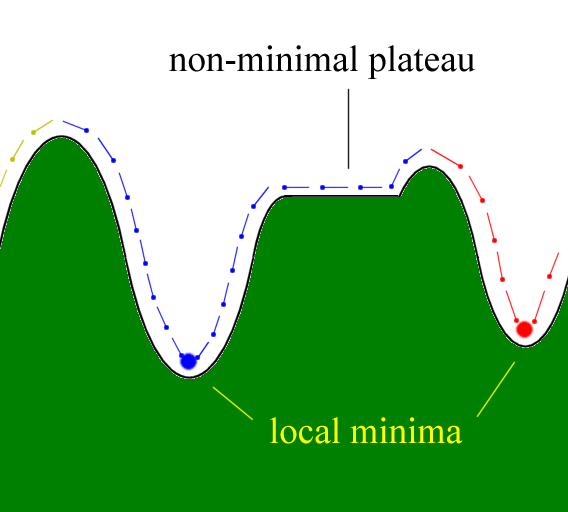
\includegraphics[height=5cm]{segmentation-watershed-rainfallingconcept-a.png}}%
	%
	\hspace{4mm}%
	%
	\subfigure[The division of the landscape into catchment basins]
	{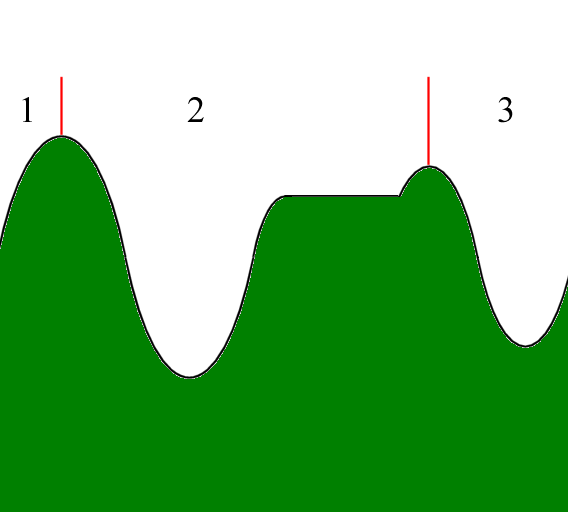
\includegraphics[height=5cm]{segmentation-watershed-rainfallingconcept-b.png}}%
\caption{The rainfalling concept of the watershed transform}
\label{fig:segmentation-watershed-rainfallingconcept}
\end{stusubfig}
%---

%---
\begin{stusubfig}{p}
	\subfigure[Beginning the flooding]
	{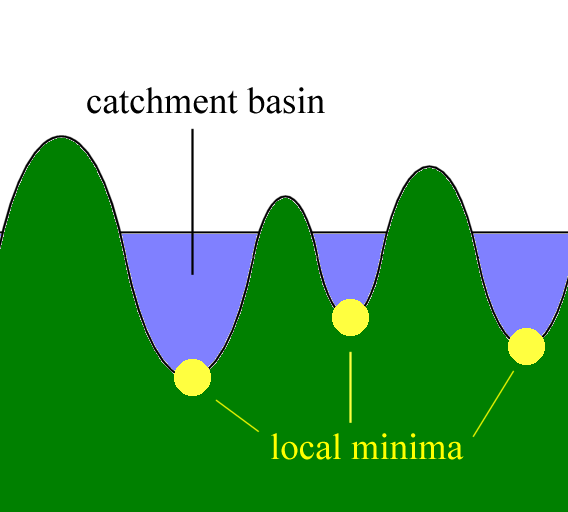
\includegraphics[height=5cm]{segmentation-watershed-floodingconcept-a.png}}%
	%
	\hspace{4mm}%
	%
	\subfigure[Two catchment basins meet]
	{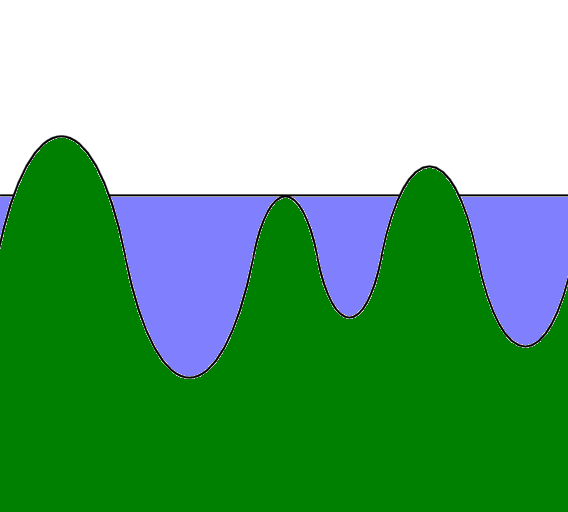
\includegraphics[height=5cm]{segmentation-watershed-floodingconcept-b.png}}%
	%
	\hspace{4mm}%
	%
	\subfigure[Building a watershed at the join point]
	{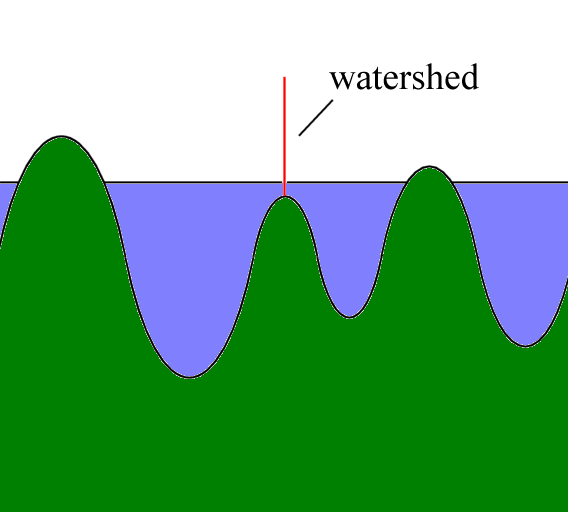
\includegraphics[height=5cm]{segmentation-watershed-floodingconcept-c.png}}%
	%
	\hspace{4mm}%
	%
	\subfigure[The division of the landscape into catchment basins]
	{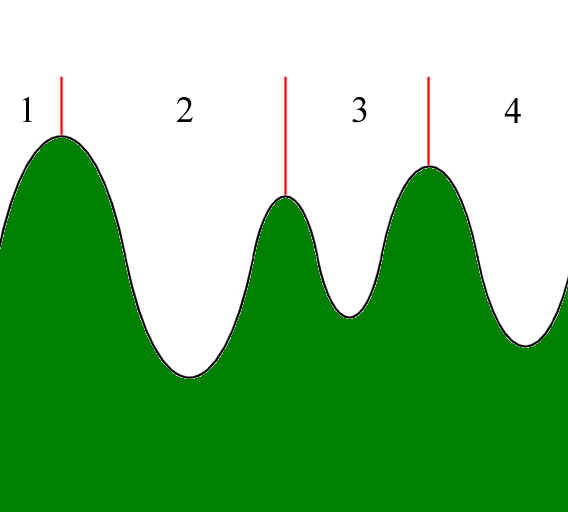
\includegraphics[height=5cm]{segmentation-watershed-floodingconcept-d.png}}%
\caption{The flooding concept of the watershed transform}
\label{fig:segmentation-watershed-floodingconcept}
\end{stusubfig}
%---

\noindent Image-based watershed algorithms produce a partition of their input into regions (see Figure~\ref{fig:segmentation-watershed-adfexample}). This can then be used for further processing.

%---
\begin{stusubfig}{t}
	\subfigure[The input image]
	{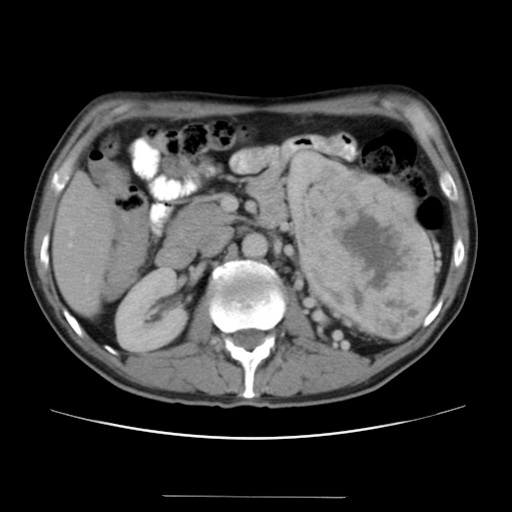
\includegraphics[height=5cm]{segmentation-watershed-adfexample-unsmoothed.png}}%
	%
	\hspace{4mm}%
	%
	\subfigure[The watershed of the image]
	{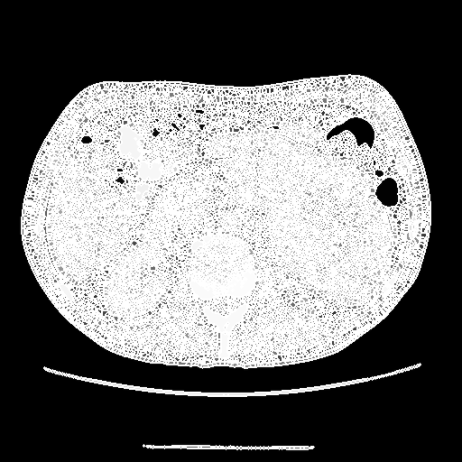
\includegraphics[height=5cm]{segmentation-watershed-adfexample-unsmoothedws.png}}%
\caption{The effects of the watershed transform. Note that the output is heavily over-segmented because the input is not smooth.}
\label{fig:segmentation-watershed-adfexample}
\end{stusubfig}
%---

\subsection{The Waterfall Transform}

In contexts where its input is not smooth (which amounts to the vast majority of real-world contexts), the watershed has an well-known and unfortunate tendency to produce an over-segmented output (again, see Figure~\ref{fig:segmentation-watershed-adfexample}). This is due to the presence of large numbers of spurious local minima in the input -- in conceptual terms, we are effectively segmenting a pock-marked landscape. The problem can be mitigated in various ways:
%
\begin{itemize}

\item The input can be smoothed (e.g.~using anisotropic diffusion filtering \cite{perona90}) before performing the watershed. This has the effect of removing some of the spurious local minima, but is usually not enough to actually solve the problem on its own. In practice, it often makes sense to smooth the image as a pre-processing step when applying hierarchical segmentation approaches -- note that this was done when producing Figure~\ref{fig:ipfs-ctconcept}, which is why the lowest partition of the image appears less over-segmented there than in Figure~\ref{fig:segmentation-watershed-adfexample}.

\item The watershed can be constrained using markers \cite{meyer90}. This directly tackles the problem by effectively specifying the desired number of output regions, but it imposes a significant manual input burden on the user.

\item The regions in the output can be iteratively merged together after finishing the watershed so as to construct a hierarchy of partitions of the input image. This does not reduce the over-segmentation of the lowest partition, but means instead that higher partitions may contain regions that are useful for later processing (e.g.~feature identification).

\end{itemize}
%
The waterfall transform is a multi-pass, hierarchical segmentation method that takes the third approach. As shown in Figure~\ref{fig:ipfs-ctconcept}, it generates a sequence of partitions of a landscape, each coarser (i.e.~containing fewer regions) than the one preceding it. Conceptually, each pass of the waterfall takes its input partition (Figure~\ref{fig:segmentation-waterfall-passconcept}(a)) and transforms it into a `stepped' landscape, where there is a step corresponding to each watershed boundary, with the height of the lowest pass point along that boundary (Figure~\ref{fig:segmentation-waterfall-passconcept}(b)). It then performs a watershed transform on this stepped landscape and outputs a coarser partition of the landscape as its result (Figure~\ref{fig:segmentation-waterfall-passconcept}(c)). This process can be repeated as long as the most recent partition has more than one catchment basin (Figures~\ref{fig:segmentation-waterfall-passconcept}(d) and (e)).

%---
\begin{stusubfig}{p}
	\subfigure[The initial partition output by the watershed]
	{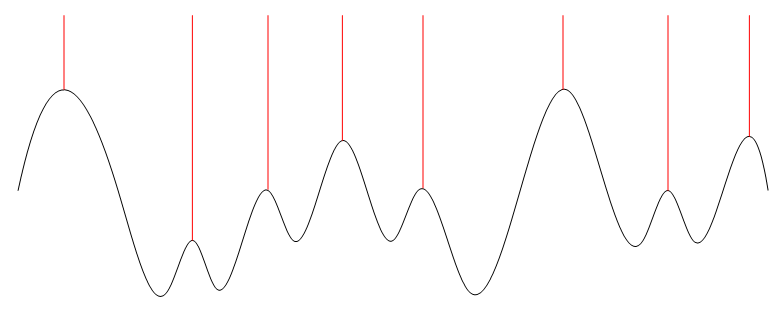
\includegraphics[height=3cm]{segmentation-waterfall-passconcept-a.png}}%
	%
	\hspace{4mm}%
	%
	\subfigure[After transforming it into a stepped landscape]
	{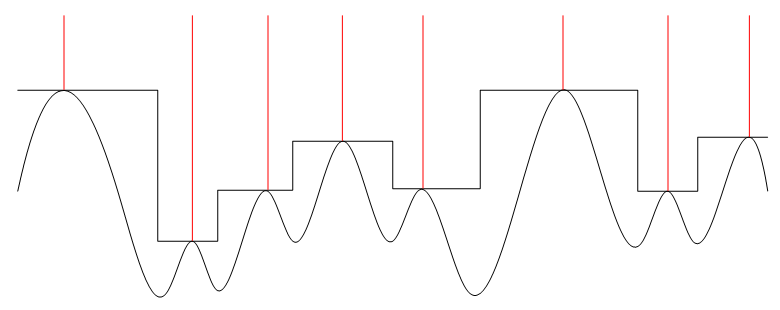
\includegraphics[height=3cm]{segmentation-waterfall-passconcept-b.png}}%
	%
	\hspace{4mm}%
	%
	\subfigure[After performing a watershed transform on the stepped landscape]
	{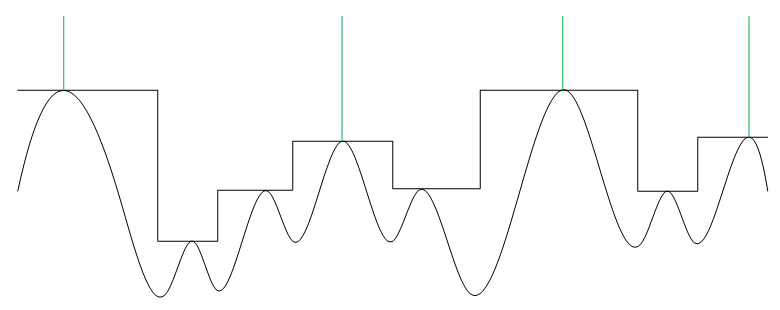
\includegraphics[height=3cm]{segmentation-waterfall-passconcept-c.png}}%
	%
	\hspace{4mm}%
	%
	\subfigure[After the second step transformation]
	{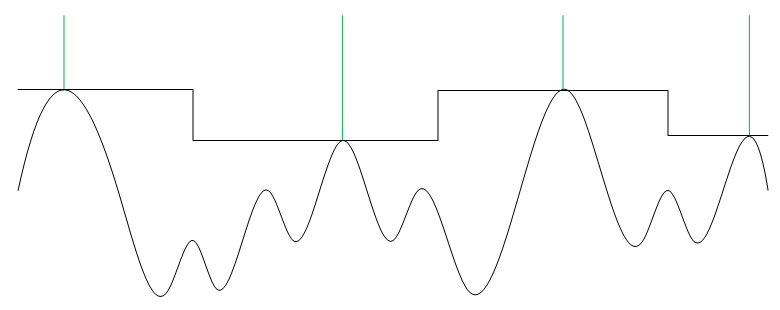
\includegraphics[height=3cm]{segmentation-waterfall-passconcept-d.png}}%
	%
	\hspace{4mm}%
	%
	\subfigure[After performing another watershed transform]
	{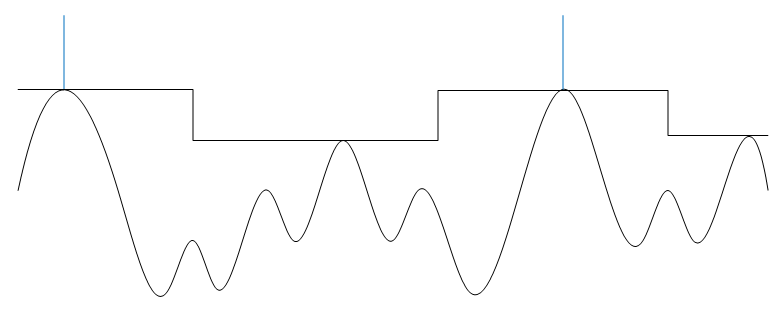
\includegraphics[height=3cm]{segmentation-waterfall-passconcept-e.png}}%
\caption{A conceptual view of the waterfall transform}
\label{fig:segmentation-waterfall-passconcept}
\end{stusubfig}
%---

\subsection{Marcotegui's Algorithm}

Whilst it is possible to perform the waterfall using the conceptual approach just described, repeatedly transforming the landscape can potentially be costly -- e.g.~image-based algorithms for the waterfall have to process all of the pixels in each region rather than just processing the region itself. This militates for alternative approaches to the waterfall based on graphs -- these can be more efficient because an entire region can be represented by a single node.

Marcotegui's algorithm \cite{marcotegui05} is a fast and effective example of such an approach. It works on a minimum spanning tree (MST) of the (weighted) region adjacency graph (RAG) of its input partition\footnotemark{}. The nodes of this graph correspond to regions in the input partition; its edges join adjacent nodes, and each edge is weighted with the height of the lowest pass point on the boundary between the nodes it joins.

\footnotetext{The justification for why an MST is sufficient can be found in \cite{marcotegui05}.}

At the start of Marcotegui's algorithm, the first input partition (produced from the input using the watershed transform) is converted into its RAG representation in a straightforward manner and an MST is built from the RAG (see \S{}A.2 of \cite{golodetz11} for implementation details). This MST is then subjected to a sequence of waterfall passes. Each waterfall pass performs a flooding-based watershed on the MST to decide which regions should be merged and elides appropriate edges in the MST to effect this (eliding an an edge means combining the nodes at either end of the edge and removing the edge itself from the MST). In detail, this involves the following steps:
%
\begin{enumerate}

\item TODO

\end{enumerate}

%---
\begin{stusubfig}{p}
  \subfigure[An example graph and its local minima (drawn in red)]
	{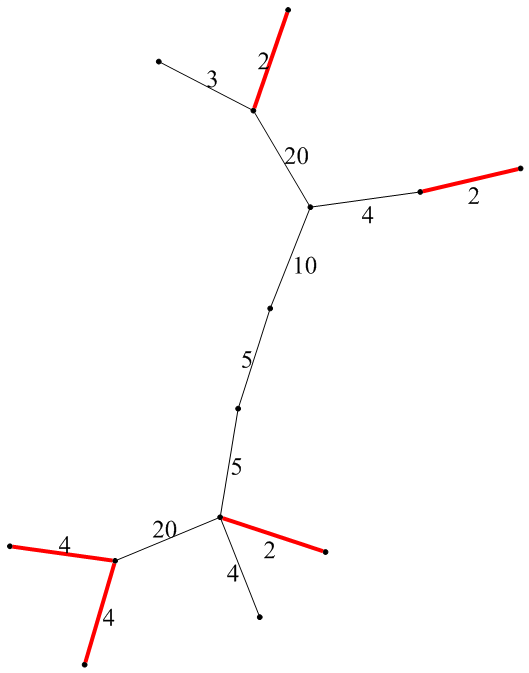
\includegraphics[width=.3\linewidth]{segmentation-waterfall-marcotegui-graphlocalminima.png}}%
	%
	\hspace{4mm}%
	%
	\subfigure[Eliding/colouring the local minima (the edges to be elided are drawn in blue)]
	{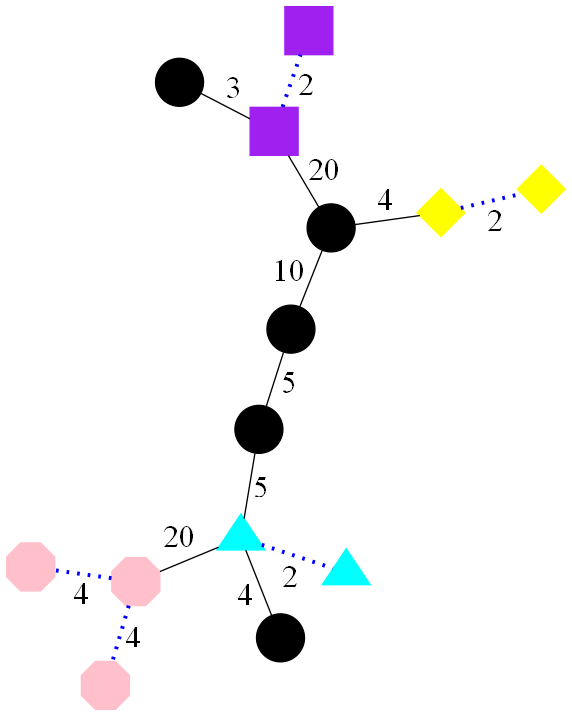
\includegraphics[width=.3\linewidth]{segmentation-waterfall-marcotegui-localminimaelision.png}}%	
\caption{Finding and eliding a graph's local minima for Marcotegui's algorithm}
\label{fig:segmentation-waterfall-marcotegui-localminima}
\end{stusubfig}
%---

%---
\begin{stusubfig}{p}
	\subfigure[Initial state]
	{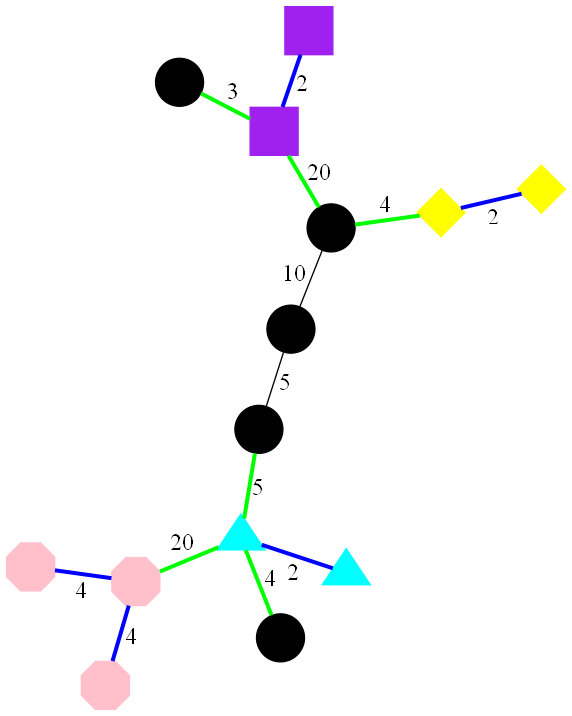
\includegraphics[width=.3\linewidth]{segmentation-waterfall-marcotegui-propagation-a.png}}%
	%
	\hspace{4mm}%
	%
	\subfigure[Elide the 3 edge]
	{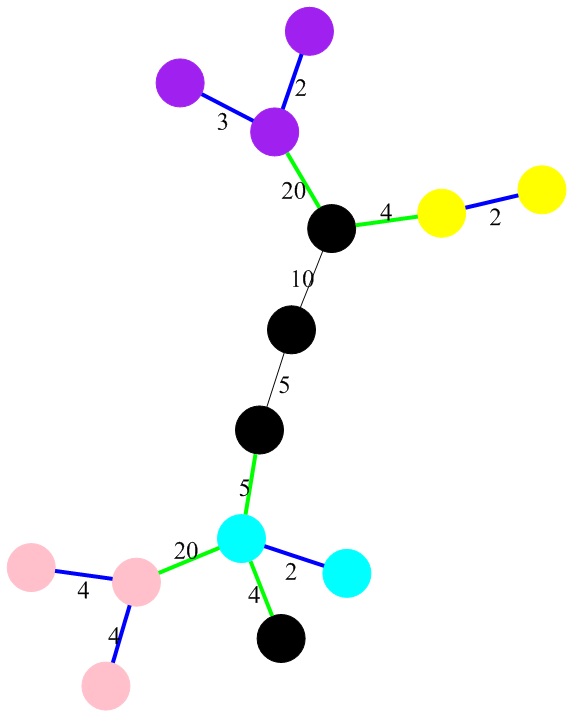
\includegraphics[width=.3\linewidth]{segmentation-waterfall-marcotegui-propagation-b.png}}%
	%
	\hspace{4mm}%
	%
	\subfigure[Elide a 4 edge]
	{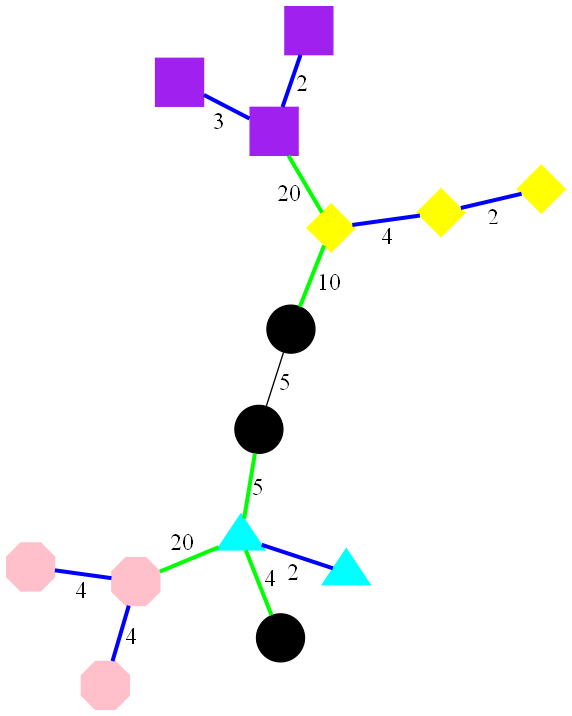
\includegraphics[width=.3\linewidth]{segmentation-waterfall-marcotegui-propagation-c.png}}%
	%
	\hspace{4mm}%
	%
	\subfigure[Elide another 4 edge]
	{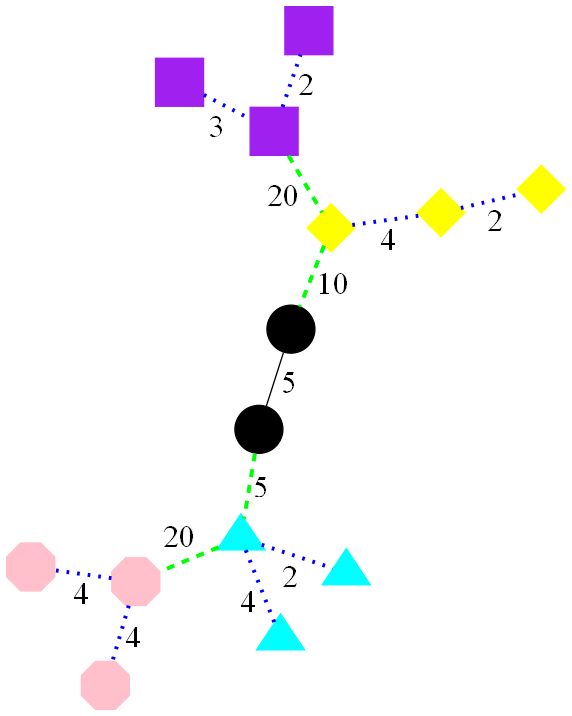
\includegraphics[width=.3\linewidth]{segmentation-waterfall-marcotegui-propagation-d.png}}%
	%
	\hspace{4mm}%
	%
	\subfigure[Elide the 5 edge]
	{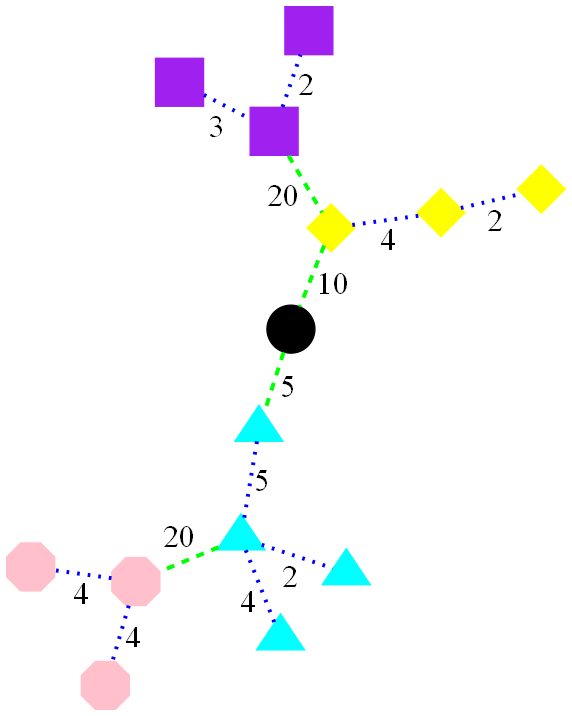
\includegraphics[width=.3\linewidth]{segmentation-waterfall-marcotegui-propagation-e.png}}%
	%
	\hspace{4mm}%
	%
	\subfigure[Elide the other 5 edge; all remaining edges will not be elided]
	{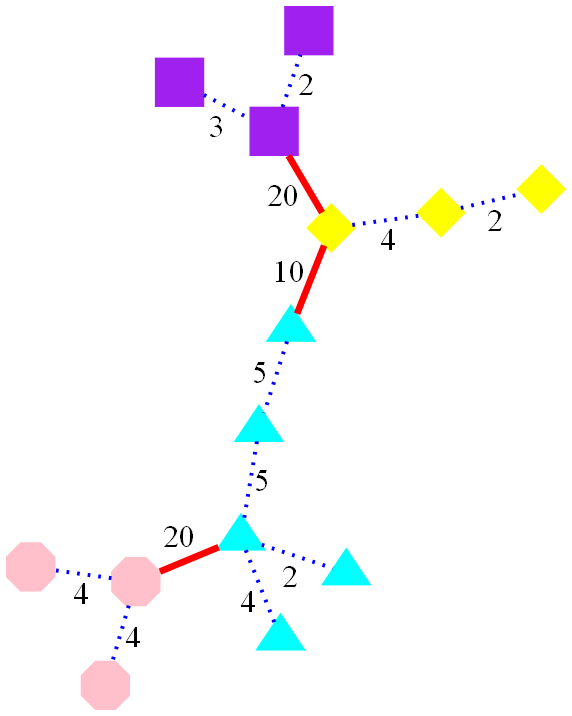
\includegraphics[width=.3\linewidth]{segmentation-waterfall-marcotegui-propagation-f.png}}%
\caption{The propagation step of Marcotegui's algorithm, illustrated on the graph in \cite{marcotegui05}: blue edges have already been elided, green edges are under consideration, and red edges will not be elided.}
\label{fig:segmentation-waterfall-marcotegui-propagation}
\end{stusubfig}
%---

%############################
\section{Nicholls' Algorithm}
\label{sec:nicholls}
%############################

TODO

%#############################
\section{Golodetz's Algorithm}
\label{sec:golodetz}
%#############################

TODO

%######################
\section{Experiments}
\label{sec:experiments}
%######################

\subsection{Segmentation Quality}

\subsubsection{Method}

TODO

\subsubsection{Results}

TODO

\subsection{Computation Time}

\subsubsection{Method}

TODO

\subsubsection{Results}

TODO

%#####################
\section{Discussion}
\label{sec:discussion}
%#####################

TODO

%######################
\section{Conclusions}
\label{sec:conclusions}
%######################

TODO

%---
\begin{stusubfig}{p}
	\subfigure[Before rooting the MST]
	{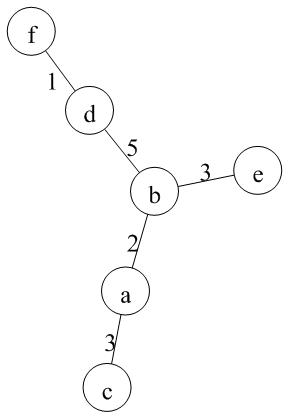
\includegraphics[height=6cm]{segmentation-waterfall-nicholls-root-before.png}}%
	%
	\hspace{4mm}%
	%
	\subfigure[After rooting it]
	{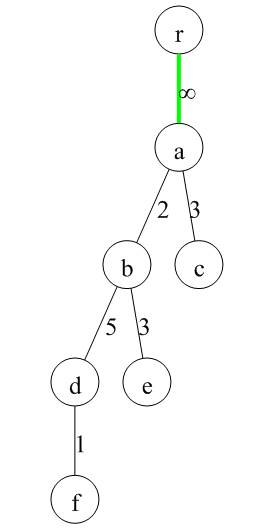
\includegraphics[height=6cm]{segmentation-waterfall-nicholls-root-after.png}}%
\caption{Nicholls' algorithm starts by picking a node at which to root the MST}% and adding a dummy root edge above the chosen root}
\label{fig:segmentation-waterfall-nicholls-root}
\end{stusubfig}
%---

%---
\begin{stusubfig}{p}
	\subfigure[The considered edge is not the unique lowest edge]
	{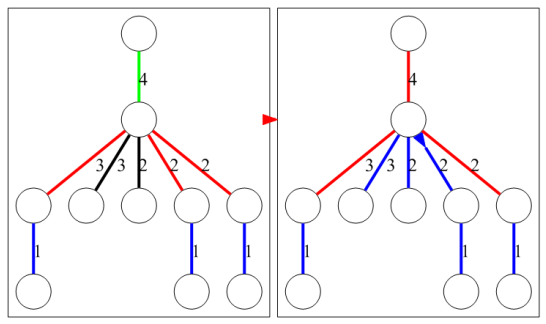
\includegraphics[height=5cm]{segmentation-waterfall-nicholls-cases-a.png}}%
	%
	\hspace{4mm}%
	%
	\subfigure[The considered edge is the unique lowest edge]
	{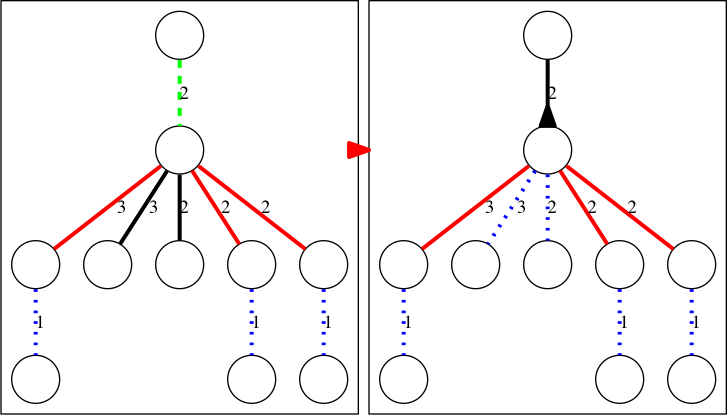
\includegraphics[height=5cm]{segmentation-waterfall-nicholls-cases-b.png}}%
\caption[Case analysis for the recursive step of Nicholls' algorithm]{Case analysis for the recursive step of Nicholls' algorithm: black edges are non-guards, red edges are guards, blue edges are those which have been elided and the green edge is the one under active consideration. The arrow (on the node) indicates the direction in which the algorithm presumes water to flow.}
\label{fig:segmentation-waterfall-nicholls-cases}
\end{stusubfig}
%---

%---
\begin{stusubfig}{p}
	\subfigure[Level 7]{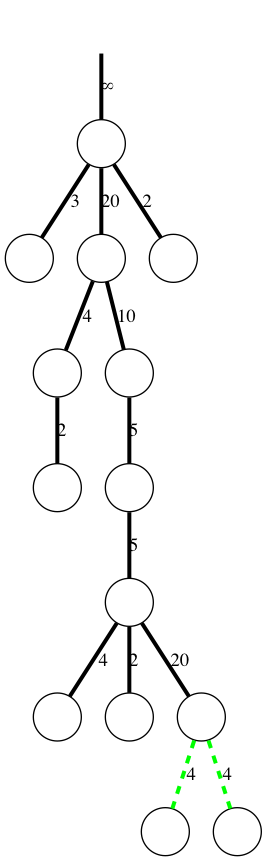
\includegraphics[width=.17\linewidth]{segmentation-waterfall-nicholls-example-a.png}}%
	\hspace{4mm}%
	\subfigure[Level 6]{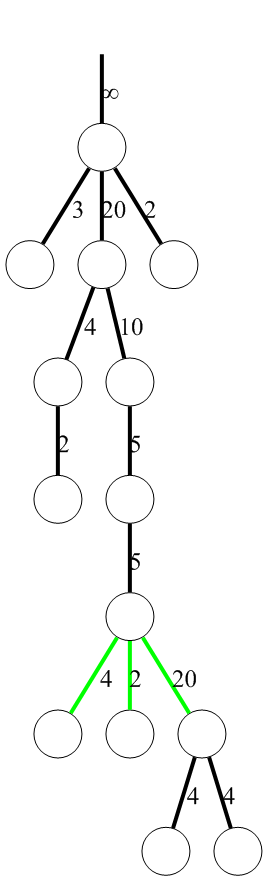
\includegraphics[width=.17\linewidth]{segmentation-waterfall-nicholls-example-b.png}}%
	\hspace{4mm}%
	\subfigure[Level 5]{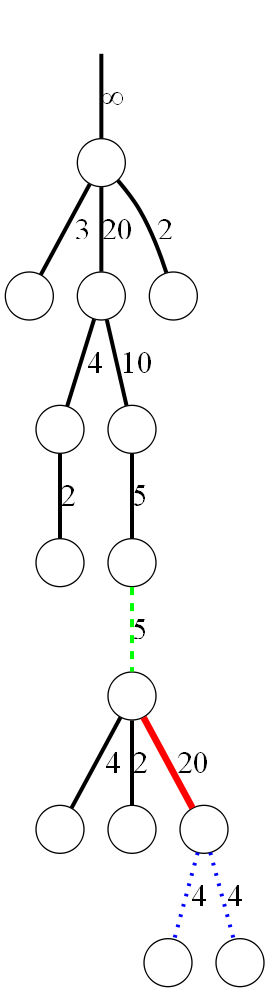
\includegraphics[width=.17\linewidth]{segmentation-waterfall-nicholls-example-c.png}}%
	\hspace{4mm}%
	\subfigure[Level 4]{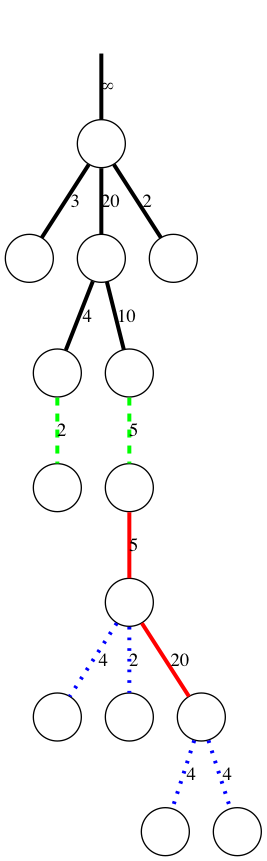
\includegraphics[width=.17\linewidth]{segmentation-waterfall-nicholls-example-d.png}}%
	\\
	\subfigure[Level 3]{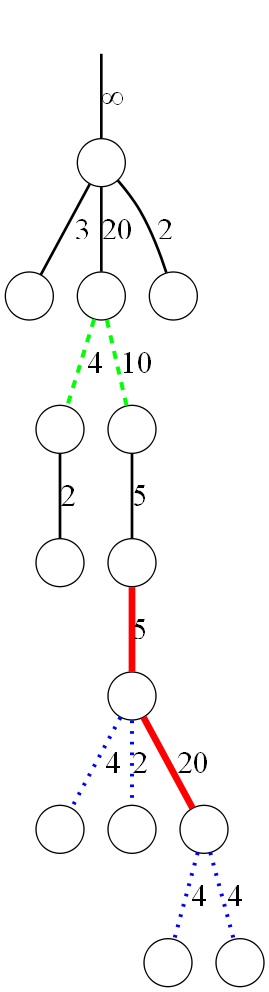
\includegraphics[width=.17\linewidth]{segmentation-waterfall-nicholls-example-e.png}}%
	\hspace{4mm}%
	\subfigure[Level 2]{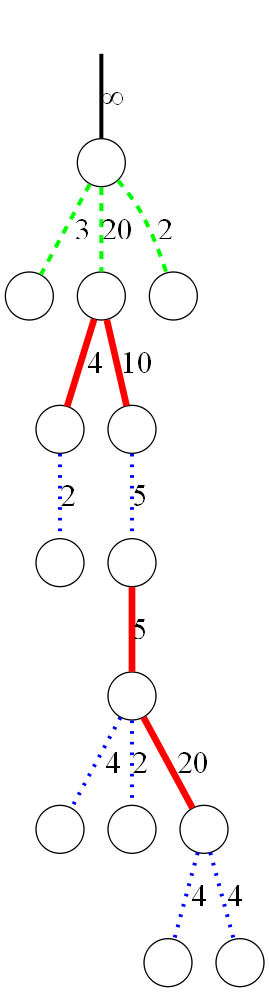
\includegraphics[width=.17\linewidth]{segmentation-waterfall-nicholls-example-f.png}}%
	\hspace{4mm}%
	\subfigure[Level 1]{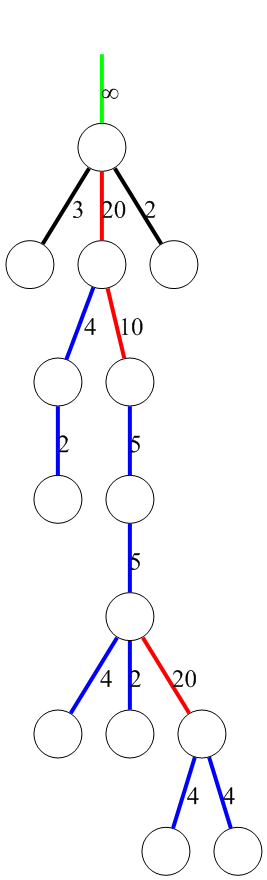
\includegraphics[width=.17\linewidth]{segmentation-waterfall-nicholls-example-g.png}}%
	\hspace{4mm}%
	\subfigure[Result]{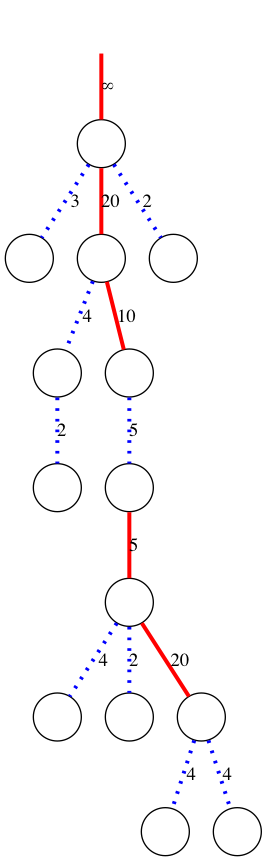
\includegraphics[width=.17\linewidth]{segmentation-waterfall-nicholls-example-h.png}}%
\caption[Nicholls' algorithm in action]{Nicholls' algorithm in action (considering all the edges in each level at a time for space reasons): black edges are non-guards, red edges are guards, blue edges are those which have been elided and green edges are ones under active consideration.}
\label{fig:segmentation-waterfall-nicholls-example}
\end{stusubfig}
%---

%---
\begin{stusubfig}{p}
	\subfigure[UI/UI]{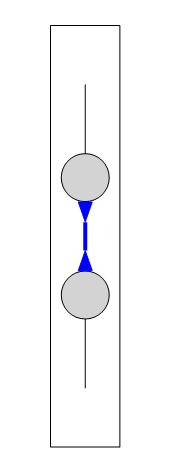
\includegraphics[height=5cm]{segmentation-waterfall-smg-mergecases-uiui.png}}%
	\hspace{4mm}
	\subfigure[UI/UO]{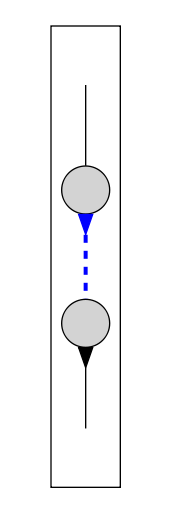
\includegraphics[height=5cm]{segmentation-waterfall-smg-mergecases-uiuo.png}}%
	\hspace{4mm}
	\subfigure[UO/AO]{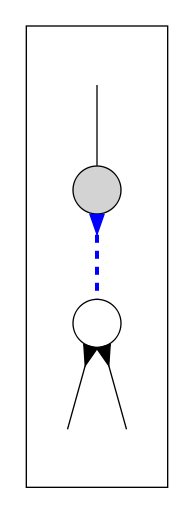
\includegraphics[height=5cm]{segmentation-waterfall-smg-mergecases-uiao.png}}%
	\hspace{4mm}
	\subfigure[UI/NF]{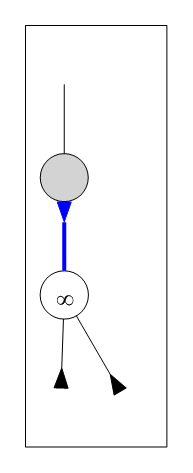
\includegraphics[height=5cm]{segmentation-waterfall-smg-mergecases-uinf.png}}%
	\hspace{4mm}
	\subfigure[NF/NF]{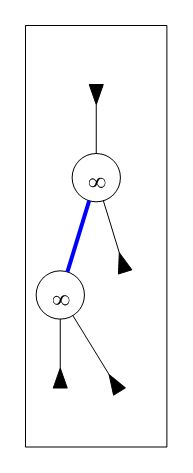
\includegraphics[height=5cm]{segmentation-waterfall-smg-mergecases-nfnf.png}}%
	\\
	\subfigure[UO/UO]{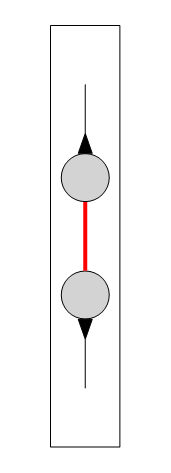
\includegraphics[height=5cm]{segmentation-waterfall-smg-mergecases-uouo.png}}%
	\hspace{4mm}
	\subfigure[UO/AI]{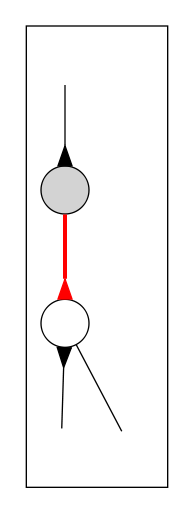
\includegraphics[height=5cm]{segmentation-waterfall-smg-mergecases-uoai.png}}%
	\hspace{4mm}
	\subfigure[UO/AO]{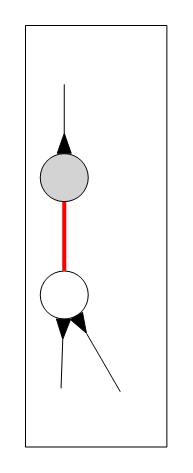
\includegraphics[height=5cm]{segmentation-waterfall-smg-mergecases-uoao.png}}%
	\hspace{4mm}
	\subfigure[UO/NF]{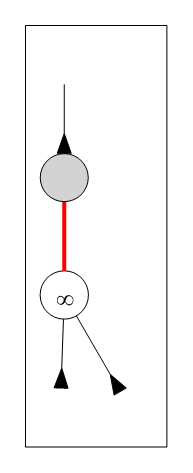
\includegraphics[height=5cm]{segmentation-waterfall-smg-mergecases-uonf.png}}%
	\\
	\subfigure[AO/AI]{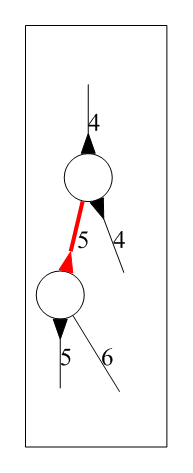
\includegraphics[height=5cm]{segmentation-waterfall-smg-mergecases-aoai.png}}%
	\hspace{4mm}
	\subfigure[AO/AO]{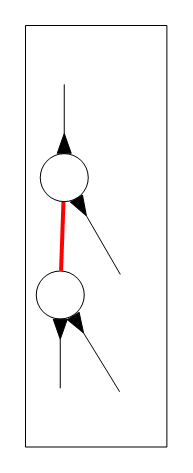
\includegraphics[height=5cm]{segmentation-waterfall-smg-mergecases-aoao.png}}%
	\hspace{4mm}
	\subfigure[NF/AI]{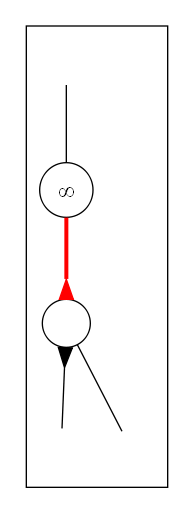
\includegraphics[height=5cm]{segmentation-waterfall-smg-mergecases-nfai.png}}%
	\hspace{4mm}
	\subfigure[NF/AO]{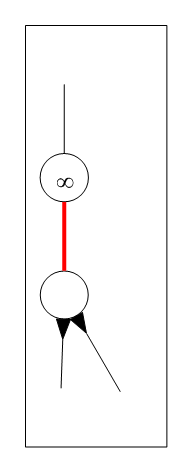
\includegraphics[height=5cm]{segmentation-waterfall-smg-mergecases-nfao.png}}%
\caption[Case analysis for the edge elision step of my waterfall algorithm]{Case analysis for the edge elision step of my waterfall algorithm (a blue edge indicates that the edge would be elided; a red edge indicates that it wouldn't). The labels are AI = ambiguous in, AO = ambiguous out, NF = no flow, UI = unambiguous in and UO = unambiguous out.}
\label{fig:segmentation-waterfall-smg-mergecases}
\end{stusubfig}
%---

%---
\begin{stusubfig}{p}
	\subfigure[The node has a unique path of steepest descent down a child edge]
	{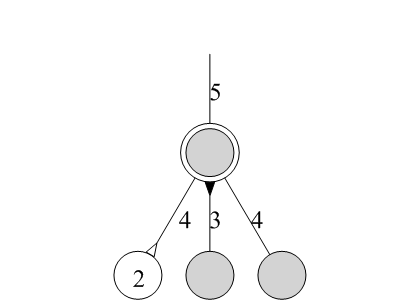
\includegraphics[width=.35\linewidth]{segmentation-waterfall-smg-pass1cases-a.png}}%
	%
	\hspace{4mm}%
	%
	\subfigure[The node has a unique path of steepest descent up the parent edge]
	{\includegraphics[width=.35\linewidth]{segmentation-waterfall-smg-pass1cases-b.png}}%
	%
	\hspace{4mm}%
	%
	\subfigure[The node has more than one path of steepest descent (and the parent edge is not a possible path of steepest descent)]
	{\hspace{8mm}\includegraphics[width=.35\linewidth]{segmentation-waterfall-smg-pass1cases-c.png}\hspace{8mm}}%
	%
	\hspace{4mm}%
	%
	\subfigure[The node has more than one \emph{downwards} path of steepest descent (but the parent edge still needs to be considered)]
	{\hspace{8mm}\includegraphics[width=.35\linewidth]{segmentation-waterfall-smg-pass1cases-d.png}\hspace{8mm}}%
	%
	\hspace{4mm}%
	%
	\subfigure[There is no flow out of the node]
	{\includegraphics[width=.35\linewidth]{segmentation-waterfall-smg-pass1cases-e.png}}%
	%
	\hspace{4mm}%
	%
	\subfigure[There is no downwards flow out of the node (but the parent edge still needs to be considered)]
	{\hspace{8mm}\includegraphics[width=.35\linewidth]{segmentation-waterfall-smg-pass1cases-f.png}\hspace{8mm}}%
\caption{Case analysis for the first pass of my waterfall algorithm}
\label{fig:segmentation-waterfall-smg-pass1cases}
\end{stusubfig}
%---

%---
\begin{stusubfig}{p}
	\subfigure[The arrow from the parent node points towards us]
	{\includegraphics[height=5.5cm]{segmentation-waterfall-smg-resolutioncases-a.png}}%
	%
	\hspace{4mm}%
	%
	\subfigure[There is no flow from the parent node]
	{\includegraphics[height=5.5cm]{segmentation-waterfall-smg-resolutioncases-b.png}}%
	%
	\hspace{4mm}%
	%
	\subfigure[There is an equally good route via the parent node]
	{\includegraphics[height=5.5cm]{segmentation-waterfall-smg-resolutioncases-c.png}}%
	%
	\hspace{4mm}%
	%
	\subfigure[There is a better route via the parent node]
	{\includegraphics[height=5.5cm]{segmentation-waterfall-smg-resolutioncases-d.png}}%
\caption[Case analysis for the resolution step of my waterfall algorithm]{Case analysis for the resolution step of my waterfall algorithm (the circled node is the one currently under consideration in each case)}
\label{fig:segmentation-waterfall-smg-resolutioncases}
\end{stusubfig}
%---

%---
\begin{stusubfig}{p}
	\subfigure[The initial tree]{\includegraphics[width=.3\linewidth]{segmentation-waterfall-smg-example-initial.png}}%
	\hspace{4mm}%
	\subfigure[After the first pass]{\includegraphics[width=.3\linewidth]{segmentation-waterfall-smg-example-pass1.png}}%
	\hspace{4mm}%
	\subfigure[After the second pass]{\includegraphics[width=.3\linewidth]{segmentation-waterfall-smg-example-pass2.png}}%
\caption[My waterfall algorithm running on a real example]{My waterfall algorithm running on a real example: the arrows on the nodes indicate the flow direction, blue edges are those that will be elided and red edges are those that won't be.}
\label{fig:segmentation-waterfall-smg-example}
\end{stusubfig}
%---

\bibliographystyle{alpha}
\bibliography{existingwork,mypapers}

\end{document}
